\chapter{Login}
\label{cha:login}

Nach erfolgreicher Registrierung und Freischaltung durch einen Administrator kann auf der Startseite der Login erfolgen. 

\noindent Über den Facebook Button kann ein \glqq oneclick\grqq ~Login ohne E-Mail und Passwort erfolgen. Beim ersten Login muss dies über einen von Facebook angezeigten Dialog erlaubt werden. Es werden zu keiner Zeit weitere Informationen weder von Facebook noch von DLRG Dienstplan ausgelesen oder auf der Facebook-Timeline gepostet. Diese Funktion dient lediglich zur Authentifizierung \cite{Facebook_Login}.

\vspace*{5mm} \noindent Über die \textit{Passwort vergessen} Funktion kann ein Link zum Passwort zurücksetzen angefordert werden. Über den zugesendeten Link kann das Passwort neu gesetzt werden.

\begin{figure}[h]
 \begin{addmargin}{-0.2\linewidth}
   \centering 
   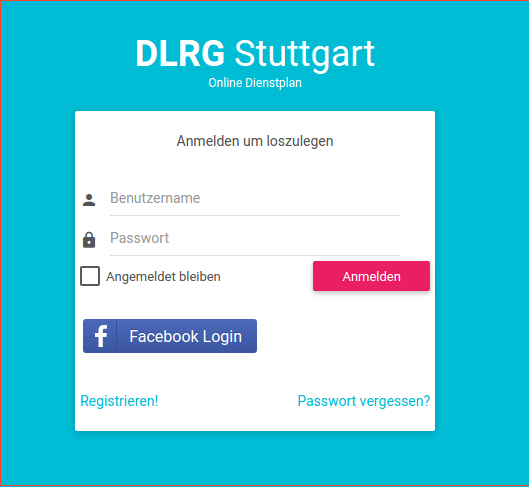
\includegraphics[width=12cm]{Bilder/view_login.png}
 \end{addmargin} 
 \caption[Login ansicht]{DLRG Dienstplan Login ansicht}
 \label{fig:view_login}
\end{figure}